\documentclass{article}
\usepackage[utf8]{inputenc}
\usepackage{graphicx}
\graphicspath{ {images/}}
\usepackage{amsthm}
\usepackage{amssymb}
\usepackage{amsfonts}
\usepackage{color}
 \usepackage{wrapfig}

\title{TP 3 \\ Equations différentielles}
\author{SABABADY Kamala et SELVARAJAH Dinusan}

\begin{document}
\maketitle

\section{{\color{red}Partie 1 :} \textit{EDO Simple}}



Pour ce devoir on a pour objectif d'apprendre à intégrer numériquement sur un intervalle $t \in [0, T]$ une équation différentielle ordinaire notée EDO. Une équation différentielle ordinaire d’ordre u est une relation entre la variable réelle $t$ , une fonction inconnue t $\mapsto u(t)$ et ses dérivées u',u'',...,$u^{(n)}$ au point t définie sous la forme :

\begin{equation}
\label{edo_0}
\color {blue}u'(t) =  f(t, u(t)),\quad u(0) = u_0
\end{equation}

Soit l'exemple de l'EDO Simple ci-dessous :

\begin{equation}
\label{exemple_1}
u'(t) =  -u(t), \quad u(0)  =  1.0
\end{equation}

Dans cet exemple la fonction f est définie par $f(t, u(t))= -u(t)$ \\

Calculons à la main la solution $u$ de l'EDO :
\begin{center}
		on a $u'(t)+u(t)=0$ \\
 	 	donc $u(t)= vect({e^{-x}}) $ \\
\end{center}

 Nous avons représenter graphiquement u à l'aide du module \textit{matplotlib}, nous avons créé le vecteur d'abscisses au moyen de \textit{numpy.linspace} et nous l'avons sauvegardé au format \textit{png} dans le répertoire courant.\\
Voici le graphique obtenue:

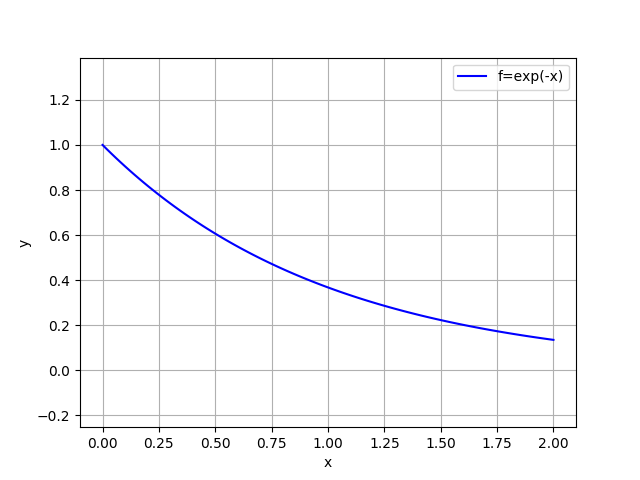
\includegraphics[width=10cm]{1.png}

\section{{\color{red}Partie 2 :} \textit{Méthode d'Euler}}


Dans cette partie, on va calculer u au moyen de la \textbf{méthode d'Euler}. En effet, on divise l'intervalle $[0, T]$ en $n$ parties égales, puis on pose $h=T/n$, ce qui fournit une subdivision $t_0 = 0, t_1 = h, t_2 = 2h, \cdots, t_n = T$. A partir de là on peut calculer approximativement la valeur de $u$ aux points $t_k$ de la subdivision et on a trouvé une approximation $u_{k+1}$ de la valeur exacte $u(t_{k+1})$ :

\begin{equation}
\label{euler}
\color{blue} u_{k+1} = u_k + hf(t_k, u_k)
\end{equation}

Si l'on connaît la valeur de la condition initiale donnée par l'EDO , on peut calculer la suite d'approximations $u_{k}$ par récurrence avec cette formule ci-dessus.
\\ 
\\
Afin de calculer les n+1 premiers termes de la suite $u_{k}$, définie par la méthode d’Euler, pour l’exemple de l'EDO Simple (2), avec $T=2.0$ et $n=10$, nous avons utilisé la formule ci-dessus avec une boucle \textbf{for} sur python.
\\
\\
Puis nous avons représenté le graphique numériquement la solution exacte $u$ et les points $(t_k,u_k)$  , voici le graphique obtenue :

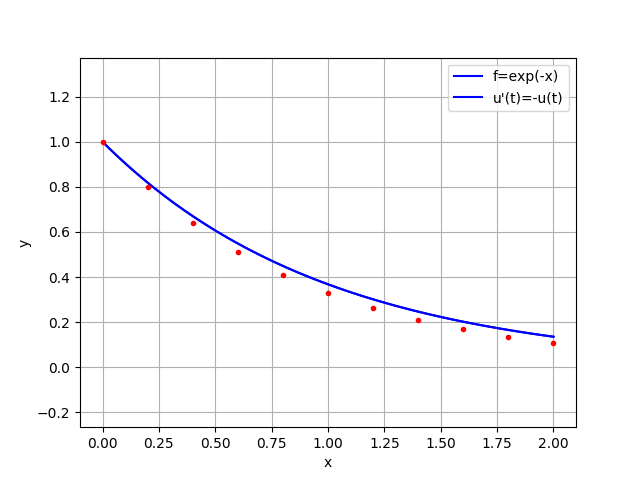
\includegraphics[width=10cm]{2.png}

\section{{\color{red}Partie 3 :} \textit{Fonction Euler Sur Python}}
\begin{wrapfigure}{l}{0.25\textwidth}
    \centering
    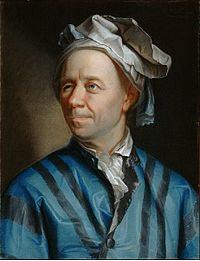
\includegraphics[width=0.25\textwidth]{euler.jpg}

\end{wrapfigure}

$$ $$

	Nous avons définie la fonction \textit{Euler} sur python  qui prend en arguments une fonction f (de deux variables scalaires) t, u, une valeur initiale $u_0$, un réel T, un entier n, et qui renvoie deux \textit{numpy arrays}: \textit{tt} de taille $n+1$, contenant les valeurs $t_k$ et $uu$ de taille $n+1$, contenant les valeurs $u_k$ obtenues par la méthode d'Euler.
\\
\\
\section{{\color{red}Partie 4 :} \textit{EDO dans Python}}

Tout d'abord nous avons définie la fonction f de l'exemple (2) sous la forme de python. Puis nous avons appliqué la fonction \textit{euler} à cet exemple et nous avons retrouvé les résultats précedents.\\
Enfin, nous avons testé notre fonction avec :
\begin{itemize} 
\item $u'(t) =  -u(t) + t,  u(0)  =  1.0$ \\ 
\item $u'(t) =  u^2(t),  u(0)  =  1.0$ \\ 
\item $u'(t) =  u^2(t) - t,  u(0)  =  1.0$
\end{itemize}
	Calculons à la main les équation différentielle ci-dessus:
\begin{enumerate}
   \item $u'(t) =  -u(t) + t,  u(0)  =  1.0$ \\
   \begin{itemize}
     \item On cherche une solution homogène de cette équation: $$ u'(t)+ u(t)=0 $$
on trouve donc $ u(t)= vect({e^{-t}})$.
     \item On cherche une solution particulier sous la forme $c(t)e^{-t}$:\\
Pour cela, on pose $u(t)= c(t)e^{-t}$ et on replace dans l'équation (1).\\
On a alors :$$ (c(t)e^{-t})' + c(t)e^{-t} = t $$
	$$<=> c'(t)e^{-t}-c(t)e^{-t}+c(t)e^{-t} = t $$
	$$<=> c'(t)=te^{t} $$
On cherche une primitive de $c'(t)$:
$$\int_{}^{} te^{t} \, \mathrm{d}t = -\int_{}^{} e^{t} \, \mathrm{d}t + [te^{t}]$$
$$\int_{}^{} te^{t} \, \mathrm{d}t = -e^{t}+te^{t}  $$
Donc la solution particulière : $(-e^{t}+te^{t})e^{-t} = t-1 $
   \end{itemize}
Donc la soulution générale est sous la forme $u(t)=ae^{-t}+t-1$ avec $a \in  \mathbb{C} $.\\
On peut trouver a avec la condition initiale: ici on a $ u(0)=1.0 $. Donc $ u(0)= a-1=1 $ $\rightarrow$ $a = 2$\\
Finalement, on a $ \color{red} u(t)= 2e^{-t} + t - 1 $
   \item $ u'(t) =  u^2(t),  u(0)  =  1.0$
On a $$ u'(t) - u^2(t)=0 $$ donc on cherche seulement la solution homogène de cette équation. 
Donc la soulution générale est sous la forme $u(t)=1/(-t+a)$ avec $a \in  \mathbb{C} $.\\
On peut trouver a avec la condition initiale: ici on a $ u(0)=1.0 $. Donc $ u(0)=1/a =1 $ $\rightarrow$ $a = 1$\\
Finalement, on a $ \color{red}u(t)= \frac{1}{1-t} $
\end{enumerate}


Mais l'équation différentielle $u'(t) =  u^2(t) - t,  u(0)  =  1.0$ ne peut pas être intégrées à la main.\\


\section{{\color{red}Partie 5 :} \textit{Intégration d'une EDO d'ordre supérieur}}

Dans cette partie, nous allons intégrer une EDO d'ordre supérieur. Prenons l'exemple:\\
\begin{equation}
\label{harmo_2}
\color{blue}u''(t) + \omega^2 u(t) = 0, \quad u(0) = u_0, \quad u'(0) = v_0 
\end{equation}
où $\omega, u_0, v_0$ sont des scalaires donnés; $\omega$ s'appelle la pulsation, $u_0$ la position initiale, $v_0$ la vitesse initiale.
Posons ensuite $v = u'$ et écrivons l'EDO sous la forme
$u'(t) =  v(t)$ et  \\
$v'(t) =  -\omega^2u(t)$ \\


Calculons à la main la solution exacte de l'EDO (4):

$$ u''(t) + \omega^2 u(t) = 0 $$ 
Cette équation admet pour équation caractéristique associée $r^2 +1 = 0$ dont les racines sont $i$ et $-i$. Les solution réelles de cette équation sont donc les fonctions de la forme t $\mapsto \cos(t)$ et $t \mapsto \sin(t)$. \\
Donc les solutions de l'équation différentielle sont les fonctions de la forme 
$$ t \mapsto A \cos(x) + B \sin(x)$$ avec $A,B \in \mathbb{C}$. \\
La condition  $u(0) = u_0$, entraîne $A = u_0 $.\\
La condition $ u'(0) = v_0 $ entraîne $B = v_0 $.\\
 Donc les solution sont $$  t \mapsto  u_0 \cos(x) + v_0 \sin(x). $$

Nous avons définit la fonction F de l'EDO (4) dans une fonction python F en choisisons $\omega = 1.0$. F prend en arguments un flottant t et un \textit{numpy atrays U} de taille 2. \\

Puis nous avons modifié la fonction \textit{euler} avec l'aide du prof pour qu'elle prenne quatre arguments : une fonction python F- elle même prenant deux arguments \texttt{t} flottant et \texttt{U} numpy array de taille $2$ -, une valeur initiale \texttt{U0} numpy array, un flottant \texttt{T} et un entier \texttt{n}; \texttt{euler} renverra deux \texttt{numpy arrays} :  \texttt{tt} de taille $n+1$, contenant les valeurs \texttt{tk}, et \texttt{UU} de taille $2\times (n+1)$, contenant les valeurs \texttt{Uk} obtenues par la méthode d'Euler.\\

Ensuite, nous avons résolue numérique ment l'EDO(4) pour cela, nous avons testé notre fonction avec $\omega = 1.0, T = 4\pi$ et les conditions initiales $u(0) = 1.0, \quad u'(0) = 0.0$. nous avons essayé avec les différentes valeurs de $n$.\\

Et enfin, nous avons représenté la solution exacte et la solution approchée donné par la méthode d'euler. En effet, on a d'abord représenté la position $u$ en fonction du temps $t$ puis la vitesse $v$ en fonction du temps $t$ et la vitesse $v$ en fonction de position $u$. \\

Voici les graphique obtenue:

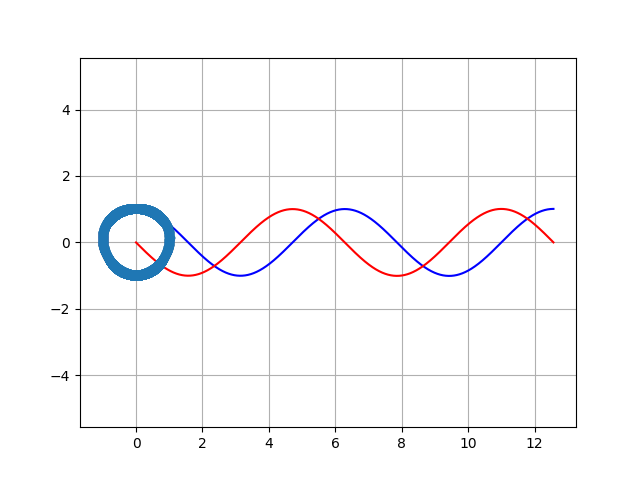
\includegraphics[width=10cm]{5.png}







\end{document}
